\chapter{Infraestructura operacional}
\label{makereference3}

El desarrollo del sistema, visto desde una perspectiva \textit{bottom-up}, comienza con la capa de abstracción más baja, correspondiente con la infraestructura operacional.

Esta infraestructura, mayormente relacionada con el apartado físico del paradigma del \gls{iiot}, integra el hardware de campo con el software de análisis y constituye el pilar fundamental del sistema. Actúa como la conexión indispensable entre los dispositivos y sensores físicos reales, la lógica abstracta del modelo de optimización matemática y la comunicación de vuelta con los resultados obtenidos.

Como es entendible, el desarrollo ha hecho uso de la infraestructura operacional ya existente en cuanto a la red interna de las instalaciones a controlar. De cualquier otro modo, el despliegue real del sistema desarrollado no hubiera sido posible, ya que se necesitarían recursos a gran escala no comúnmente disponibles, pudiendo visualizar el activo energético principal en cuestión en la figura~\ref{fig:diagrama-bess}.

\begin{figure}
  \centering
  \includesvg[width=0.5\linewidth]{figures/diagrama-bess.svg}
  \caption[Diagrama de un sistema de almacenamiento de energía en baterías.]{Diagrama de un sistema de almacenamiento de energía en baterías~\cite{iberdrola2024bess}.}
  \label{fig:diagrama-bess}
\end{figure}

Por ello, la principal contribución del apartado de la infraestructura operacional se ve reflejada en la configuración, securización, despliegue y validación de la herramienta de conexión entre los activos físicos y del historiador del \gls{pis}, a través de los correspondientes protocolos de comunicación posteriormente descritos. Se busca la integración estandarizada con los componentes ya existentes, para el correcto funcionamiento de las instalaciones que alojan los \glspl{bess}, mientras se tiene en cuenta que los sistemas de almacenamiento apenas son una pequeña parte de la red al completo.

De esta forma, es posible obtener una visión más completa a través del análisis realizado en la sección~\ref{makereference3.1}, que define la arquitectura de la disposición de los activos energéticos y las múltiples restricciones operativas fundamentales tenidas en cuenta por el desarrollo. También, se examinan los componentes físicos que forman parte de la infraestructura al completo, detallados en la sección~\ref{makereference3.2}, que actúan como la fuente primaria de la obtención de datos. Además, se explora la comunicación que unifica estos componentes en la sección~\ref{makereference3.3},  facilitando un intercambio de datos estandarizado. Con esto, se describe la gestión de la información obtenida en la sección~\ref{makereference3.4}, detallando su rol en el almacenamiento, la gestión y la validación de los datos operativos. Por último, se explica como los datos de la infraestructura obtenidos son transformados y consumidos en la sección~\ref{makereference3.5}.

\section{Configuración topológica}
\label{makereference3.1}

Resulta que en los \glspl{bess}, la efectividad operativa y la rentabilidad, esta última sobre todo, no dependen exclusivamente de la tecnología intrínseca utilizada o de la optimalidad de su operación, sino que están condicionadas fundamentalmente por su configuración topológica.

Esta disposición es absolutamente necesaria para llegar a comprender el funcionamiento de la representación operacional de las plantas, ya que una de las principales motivaciones del desarrollo del sistema ha resultado ser la intención de aprovechar las ventajas de que brindan las topologías más avanzadas e integradas con el resto de activos, como lo es la topología híbrida aquí descrita. Posteriormente, en el apartado~\ref{makereference5} de modelización estructural se describe la implementación de la lógica topológica y en el apartado~\ref{makereference7} de resultados experimentales las diferencias en la operación de las topologías.

Así, la topología de una instalación energética se refiere a la arquitectura física de conexión de los activos energéticos con la red eléctrica y otros elementos de generación o consumo dentro de la instalación misma en todo su conjunto~\cite{parlikar2019topology}.

Esta define los flujos energéticos posibles y, por ello, impone las restricciones estructurales que el modelo de optimización debe considerar como premisas inviolables para garantizar la validez física y económica de las soluciones.

Precisamente, estos flujos energéticos son los que dictan los canales de importación y exportación de energía entre la red pública de alta tensión, controlada por el \gls{tso}, y la red interna de media tensión de la entidad energética, manejadas las instalaciones de almacenamiento mismas por el control del sistema desarrollado, a través del llamado \gls{pf}.

De igual manera, es necesario subrayar la relevancia de los flujos energéticos nuevamente, ya que todas y cada una de las operaciones en el mercado se realizan a través ellos, cada uno poseyendo una identificación correspondiente al flujo energético pertinente, como se muestra en la tabla~\ref{tab:unidades-fisicas}.

\begin{table}[ht]
  \centering
  \begin{tabular}{|l|l|l|l|}
    \hline
    UFI     & UP      & UOF     & Descripción         \\
    \hline
    BPLLANC & AFIBHFC & AFIBHFC & Batería Compra      \\
    BPLLANV & FBHIBHV & IBEVD22 & Batería Venta       \\
    PLLANO  & FBHIBHV & IBEVD22 & H.B. Puertollano II \\
    BURKIC  & AFIBHEC & AFIBHEC & Batería Compra      \\
    BURKIV  & EBHIBHV & IBEVD24 & Batería Venta       \\
    ELGURKI & EBHIBHV & IBEVD24 & P.E. Elgea-Urkilla  \\
    \hline
  \end{tabular}
  \caption[Unidades físicas, de programación y de oferta.]{Unidades físicas, de programación y de oferta de múltiples instalaciones.}
  \label{tab:unidades-fisicas}
\end{table}

Los flujos energéticos, o, mejor expresado, las interfaces correspondientes a los mismos, son conocidos como \gls{ufi}, mientras que la interfaz que oferta a mercado y engloba las \glspl{ufi} es llamada \gls{up} desde el punto de vista del \gls{tso} y \gls{uof} desde la perspectiva del \gls{mo}.

El sistema desarrollado, por tanto, hace uso de la configuración topológica ya existente, es decir, no se encarga de la implantación física de los activos energéticos o de la conexión de los mismos con la red física, ya que eso queda bien fuera del alcance del diseño. En cambio, sí que hace uso de los diferentes componentes mediante sus correspondientes canales.

De esta forma, en términos generales y en el ámbito del mercado eléctrico peninsular, como es el caso, las instalaciones que alojan baterías de escala industrial se pueden clasificar principalmente en dos grandes familias, la configuración aislada y la híbrida, basada la terminología en las definiciones oficiales del Estado~\cite{cnmc2024servicios}.

\subsection{Topología aislada}
\label{makereference3.1.1}

La configuración aislada o \textit{standalone} representa el arquetipo más directo de despliegue de un \gls{bess}~\cite{gallo2023stand}.

En esta topología, la batería es el único activo energético de la instalación y su principal propósito es interactuar con la red eléctrica pública de alta tensión, conectada a través del \gls{pf} a la red interna de media tensión, como se observa en la figura~\ref{fig:topologia-aislada}.

\begin{figure}
  \centering
  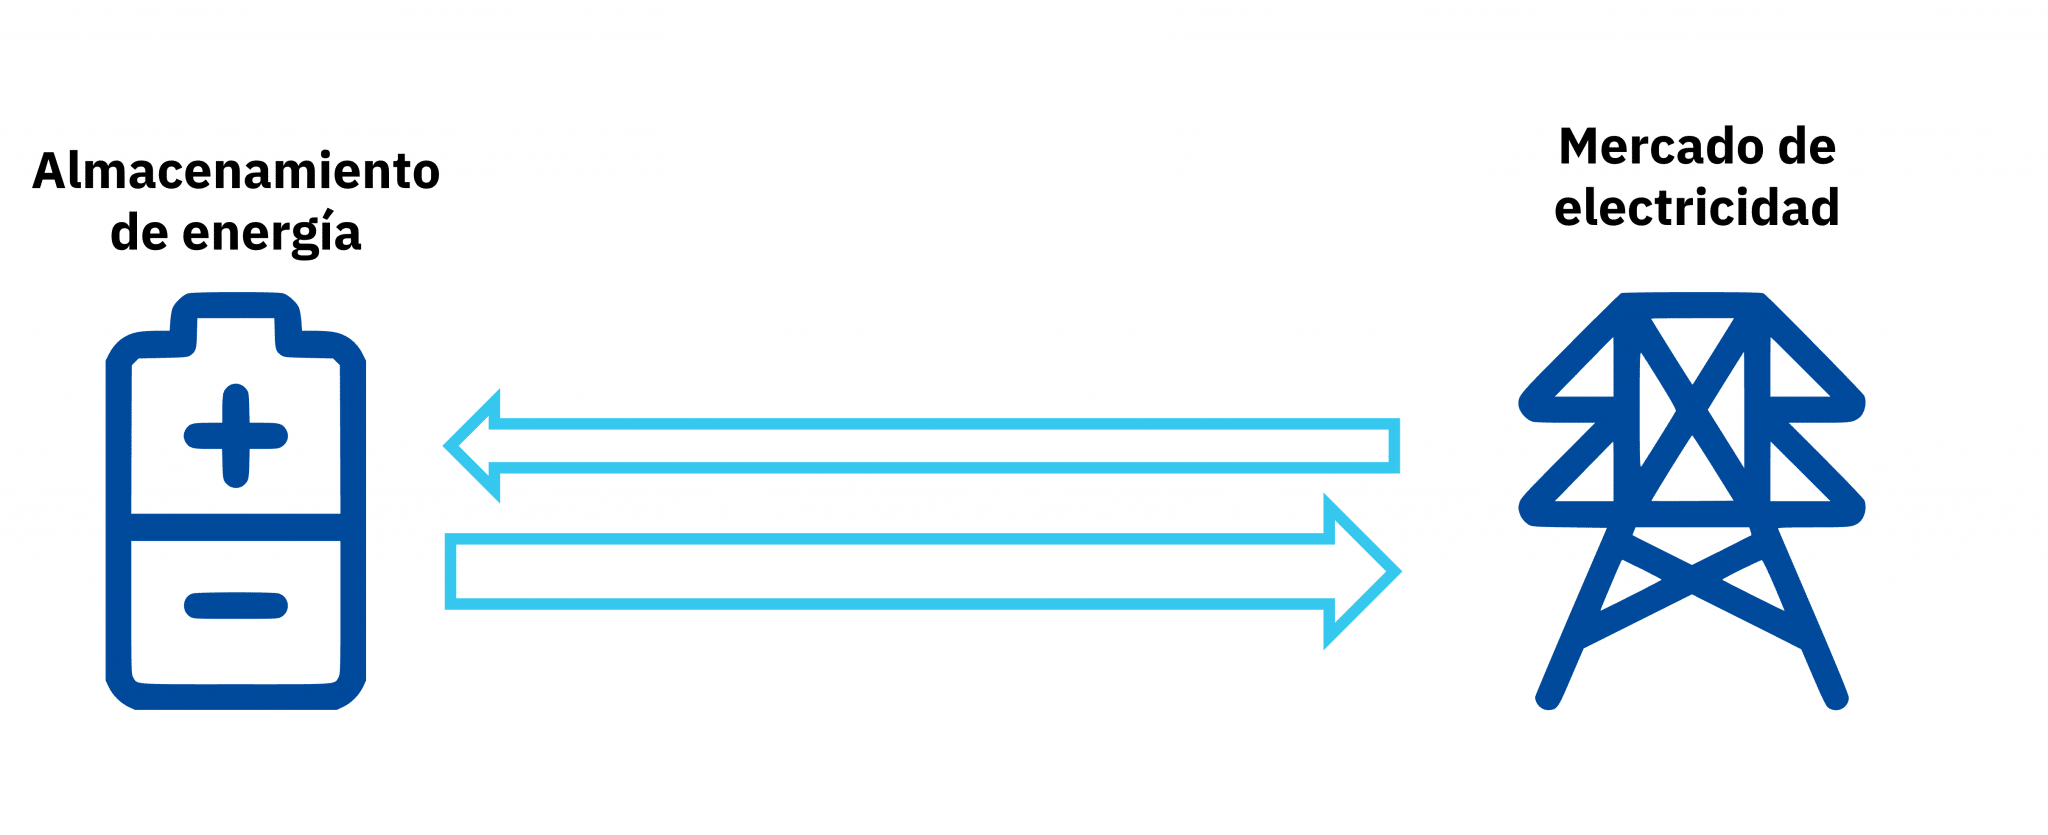
\includegraphics[width=0.5\linewidth]{figures/topologia-aislada.png}
  \caption[Diagrama de una instalación aislada.]{Diagrama de una instalación aislada con su activo de almacenamiento y sus correspondientes flujos energéticos~\cite{aleasoft2025la}.}
  \label{fig:topologia-aislada}
\end{figure}

Esto significa que la operación de un sistema de almacenamiento de energía en baterías aislado se centra puramente en el intercambio de energía con la red, lo que tan solo permite definir dos interfaces de flujo energético.

\begin{itemize}

  \item La interfaz de importación se corresponde al flujo de energía desde la red hacia el \gls{bess}. Este flujo comprende la única fuente de carga de la batería.

  \item  La interfaz de exportación representa el flujo de energía desde el \gls{bess} hacia la red. En contrapunto, se corresponde con la descarga de la batería.

\end{itemize}

De esta forma, esta topología es más común en las instalaciones energéticas principalmente dedicadas al negocio en los mercados de ajuste~\cite{carbajo2007mercados}, de tal forma que no necesiten encargarse del aprovechamiento energético de otros posibles activos energéticos dentro de la misma instalación.

Precisamente, uno de los ejemplos más representativos de esta topología en la actualidad es el \gls{bess} de Abadiño, en donde el negocio principal se realiza en los mencionados mercados de ajuste (las diferencias entre la situación actual y futura de las instalaciones standalone resulta especialmente interesante y es evaluada posteriormente en la sección~\ref{makereference7.3}).

A pesar de su aparente simplicidad, los análisis de mercado demuestran que la viabilidad económica de la topología aislada es limitada~\cite{azahra2020optimized, baviskar2023opportunities, kalenderova2024batery}.

El margen diferencial de precios, también conocido como \textit{spread}, entre las horas de bajo coste (valle) y alto coste (pico), a menudo resulta insuficiente para generar los ingresos necesarios que permitan amortizar la elevada inversión de capital y cubrir el \gls{capex} y \gls{opex}, incluyendo la degradación.

De hecho, para que estas instalaciones sean rentables, generalmente deben diversificar sus fuentes de ingresos mediante la participación activa en los dichos mercados de servicios de ajuste, como el \gls{afrr} y el \gls{mfrr}, teniendo que ofrecer disponibilidades de frecuencia y potencia.

Aunque la participación en estos mercados de regulación ofrezca una remuneración por la disponibilidad de capacidad, lo que se adapta perfectamente a la rápida respuesta de conmutación de las baterías, proporciona flujos de ingreso inestables de cara al futuro. Esto es debido al enorme crecimiento de la implantación de sistemas de almacenamiento de energía en baterías esperado, aumentando la oferta de disponibilidad y, por lo tanto, reduciendo a su vez las ganancias generadas individualmente por las baterías.

Cabe destacar que, aun teniendo una baja rentabilidad esperada, el sistema desarrollado soporta la configuración aislada sin ninguna complicación, al ser diseñado con una arquitectura modular en mente, capaz de adaptarse a, presuntamente, cualquier configuración topológica.

\subsection{Topología híbrida}
\label{makereference3.1.2}

Con el propósito de superar las limitaciones del modelo aislado y maximizar el aprovechamiento de la energía, han emergido con fuerza las configuraciones híbridas~\cite{bresciani2025hybridization}, el principal enfoque del sistema.

Estas topologías se definen por la llamada colocación del activo de generación, principalmente de generación renovable y generalmente fotovoltaica o eólica, con un \gls{bess}, como se muestra en la figura~\ref{fig:topologia-hibrida}.

\begin{figure}
  \centering
  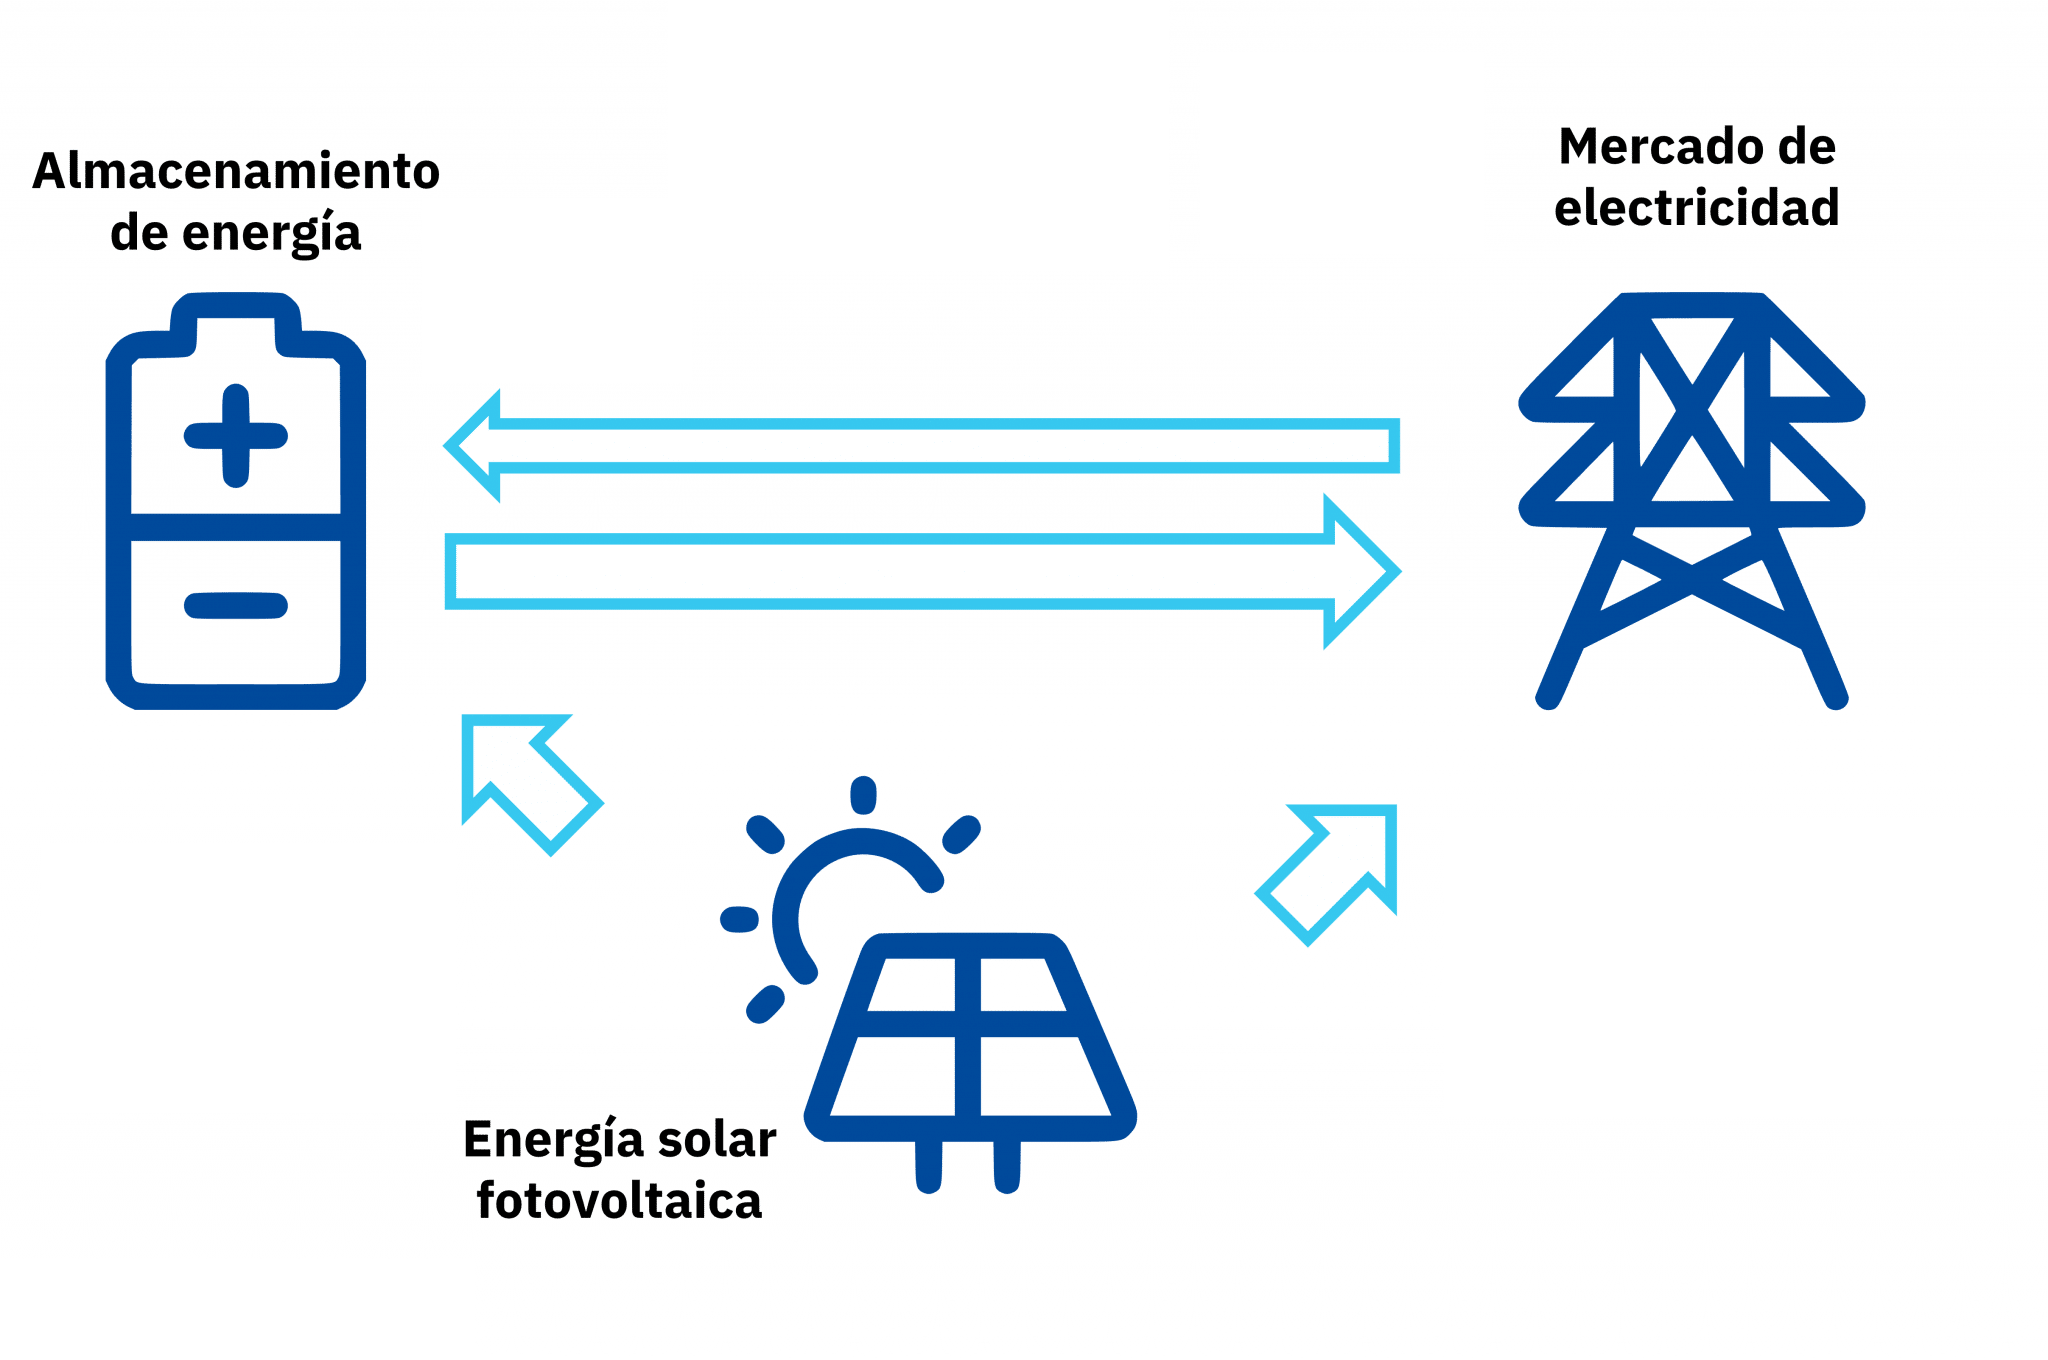
\includegraphics[width=0.5\linewidth]{figures/topologia-hibrida.png}
  \caption[Diagrama de una instalación híbrida.]{Diagrama de una instalación híbrida con sus activos de almacenamiento y generación y sus correspondientes flujos energéticos~\cite{aleasoft2025la}.}
  \label{fig:topologia-hibrida}
\end{figure}

Aunque los activos energéticos compartan ambos el mismo \gls{pf}, desde donde importan o exportan la energía a la red eléctrica, la batería es capaz de operar mediante lo que se conoce como \textit{behind the meter}. Esto es porque el flujo energético se mantiene dentro de la red interna de media tensión, sin volcarse necesariamente a la red pública de alta tensión.

\begin{itemize}

  \item Las interfaces de importación se corresponden tanto al flujo de energía desde la red hacia el \gls{bess} como al flujo energético desde la generación energética al \gls{bess}. Más allá de posibles restricciones estructurales u operativas, el sistema desarrollado debe ser capaz de diferenciar y seleccionar correctamente el canal de importación más adecuado según la situación analizada.

  \item Las interfaces de exportación representan, por un lado, el flujo de energía desde el \gls{bess} hacia la red, y por el otro, el flujo de energía desde la generación energética a la red. Como se tratan de dos activos energéticos separados, el desarrollo debe tenerlos en cuenta a los dos a la hora de realizar el arbitraje y dar la opción de comunicar no solo los resultados de la batería, sino también los de la generación, al estar enlazados entre sí, como se detalla en la sección~\ref{makereference5.3}.

\end{itemize}

Esta capacidad de carga interna transforma bastante notablemente el modelo operativo. Sin embargo, el término de hibridación mismo no describe un modelo único, ya que las restricciones operativas varían entre instalaciones, lo cual exige una flexibilidad muy grande por parte del funcionamiento del sistema desarrollado.

Por ello, la herramienta identifica y soporta de forma genérica las siguientes operaciones de la topología híbrida.

\begin{description}

  \item[Híbrida flexible] La configuración más versátil. El sistema de control tiene total libertad para decidir la fuente de carga (red eléctrica o generación energética) basándose exclusivamente en el criterio óptimo del algoritmo de control, que principalmente se trata de la maximización del beneficio. La instalación híbrida fotovoltaica y de almacenamiento de Puertollano es un arquetipo de este modelo.

  \item[Híbrida con prioridad de carga de generación] Opera bajo una restricción no económica, es decir, debe sacrificar beneficio para cumplir con las limitaciones del funcionamiento físico de la instalación. Una norma operativa de naturaleza física, aunque también pueda ser contractual o regulatoria, obliga al \gls{bess} a absorber toda la energía generada por la planta antes de poder cargar desde la red. La planta de híbrida eólica y de almacenamiento de Urkilla ejemplifica este tipo de limitación.

  \item[Híbrida con carga aislada de la red] Representa el escenario más restrictivo. La interfaz de importación desde la red para la carga del \gls{bess} está física o lógicamente deshabilitada, siendo la planta renovable asociada la única fuente de carga. Este modelo limita la operación a estrategias de autoconsumo de la producción renovable, donde se puede llegar a reservar parte de la generación para la batería. La instalación híbrida fotovoltaica y de almacenamiento de Campo Arañuelo es una representación de esta configuración.

\end{description}

La hibridación, incluso en sus formas más restrictivas, ofrece ventajas comparativamente altamente decisivas. Resulta que permite maximizar el valor de la energía renovable, almacenando excedentes que de otro modo se verterían a coste nulo. Además, al cargar desde la fuente renovable local, se evitan los costes regulatorios asociados al uso de la red pública~\cite{mterd2024orden} (peajes y cargos como el IVPEE, el bono social o las subvenciones del operador del sistema), lo que representa un ahorro directo y sustancial que mejora drásticamente los márgenes de arbitraje.

\section{Instrumentación de campo}
\label{makereference3.2}

La instrumentación de campo constituye el conjunto de dispositivos físicos que actúan como la interfaz directa entre los flujos energéticos. Por un lado, se encargan de medir con precisión las variables físicas clave (como la potencia, tensión, \gls{soc}, etc.) y por otro, son los actuadores que ejecutan las órdenes generadas por la lógica de control y optimización.

Concretamente, a partir dichos componentes, \gls{bms}, \gls{pcs}, transformador de medida y \gls{rtu}, ofrecidos por entidades como CATL~\cite{catl2023catl} e Ingeteam~\cite{ingeteam2025ingeteam}, el sistema extrae las siguientes señales.

\begin{description}

  \item[Estado de carga] Indica el porcentaje de energía en la batería. Es la variable más crítica para la toma de decisiones de carga y descarga. Expresado en porcentaje y megavatios hora\footnote{Dependiendo de la batería, aún todas siendo del mismo fabricante, es expresado de un modo u otro, por alguna razón.} y ofrecido por el \gls{bms}.

  \item[Estado de salud] Representa la capacidad actual de la batería en comparación con su capacidad nominal, reflejando su nivel de degradación a lo largo del tiempo. Expresado en porcentaje y megavatios hora\footnotemark[\value{footnote}] y ofrecido por el \gls{bms}.

  \item[Límites de potencia de carga y descarga local] Potencia máxima que el sistema de almacenamiento de baterías puede admitir o entregar en un momento dado, la cual puede estar limitada por factores internos como la temperatura. Expresados en megavatios y ofrecido por el \gls{bms}.

  \item[Disponibilidad] Señalización de la disponibilidad del estado interno de la batería, en forma de la cantidad de módulos o conjunto de celdas de carga disponibles en un momento dado, dependiendo de posibles fallos en la operación del sistema de almacenamiento. Expresado en porcentaje y ofrecido por el \gls{bms}.

  \item[Programa] El valor de consigna que el \gls{bms} está intentando seguir actualmente. Expresado en megavatios y ofrecido al \gls{bms}.

  \item[Potencia activa de carga y descarga] Medida en tiempo real de la potencia neta que se está inyectando o absorbiendo de la red. Expresado en megavatios y ofrecido por el \gls{pcs}.

  \item[Potencia activa de importación y exportación] La medición física de la potencia bruta que fluye a través del punto frontera, siempre dentro de la red de media tensión. Expresado en megavatios y ofrecido por los transformadores de medida.

  \item[Límites de potencia de descarga global] La máxima potencia de descarga que la planta puede ofrecer en su conjunto, la también llamada potencia estructural, que debe ser comunicada previamente al \gls{tso} por consideraciones legales. Expresados en megavatios y ofrecido por el \gls{rtu}.

  \item[Modo de control actual] Indica si la planta opera siguiendo las consignas externas señalizadas por el sistema a través del programa, o automáticamente por su cuenta según modos de funcionamientos internos no usados en el proyecto. Ofrecido por el \gls{rtu} y se fija en el seguimiento del programa.

\end{description}

De tal forma, estas son las señales de entrada y salida comunicadas a través de los protocolos de comunicación descritos en la siguiente sección~\ref{makereference3.3}, las cuales deparan en el sistema de información de planta de la sección~\ref{makereference3.4} tras ser adecuadamente configuradas.

\section{Protocolos de comunicación}
\label{makereference3.3}

Una vez los sensores han medido las variables físicas, los datos deben transmitirse de manera fiable y estructurada generalmente hasta la plataforma central o, en este caso, al \gls{pis}.

Para ello es necesario llevar a cabo una correcta selección de los protocolos de comunicación industriales a utilizar, siendo esta una de las tareas realizadas en el ámbito de la comunicación fuera de los activos de la instalación interna.

El principal desafío en entornos industriales es la interoperabilidad, siendo esta la capacidad de los diferentes dispositivos de intercambiar información sin ambigüedades. Por eso, los protocolos de comunicación son las reglas que actúan como el formato común para lograr esta necesaria interoperabilidad.

De esta forma, el \gls{pis}, explicado más adelante en la sección~\ref{makereference3.4}, debe entablar un vínculo con el controlador de planta o \gls{rtu}, concretamente. Pero, a la misma vez, el \gls{rtu} mismo necesita interactuar con el resto de activos físicos si pretende controlarlos de forma precisa.

Esa es la razón de la exposición de múltiples protocolos, y es que la comunicación entre los activos energéticos y el \gls{rtu} se realiza mediante Modbus TCP de forma agnóstica al sistema desarrollado, mientras que la comunicación entre el \gls{rtu} y el \gls{pis} es a través de IEC 60870-5-104.

\begin{figure}
  \centering
  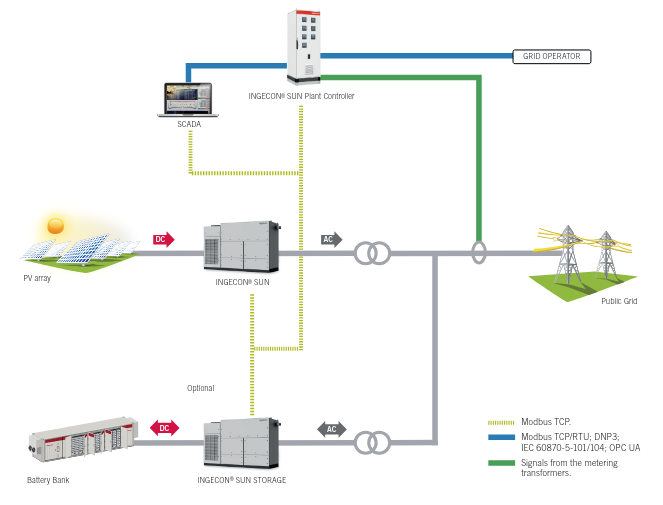
\includegraphics[width=0.5\linewidth]{figures/instrumentacion-de-campo.png}
  \caption[Diagrama de instrumentación de campo.]{Diagrama de la interacción entre los dispositivos y sensores físicos de campo.}
  \label{fig:instrumentacion-de-campo}
\end{figure}

\subsection{Modbus TCP}
\label{makereference3.3.1}

Modbus es uno de los estándares de facto en la automatización industrial por su simplicidad. Generalmente, es considerado uno de los estándares de comunicación industrial más ampliamente soportados~\cite{swales1999open}.

El protocolo sigue un modelo de comunicación conocido como maestro-esclavo, donde un dispositivo cliente (maestro) inicia las transacciones enviando peticiones a los dispositivos servidores (esclavos) para leer o escribir datos. Permite la interacción simple con sus relés, registros de entrada, registros de consigna y entradas discretas.

Los servidores responden a estas peticiones, asegurando un intercambio de información estructurado y fiable. Modbus TCP es precisamente ampliamente utilizado para la comunicación en la industria, al utilizar, como su propio nombre indica, el protocolo de capa de transmisión TCP/IP internamente. Ventajosamente, no requiere de lazos físicos entre los activos.

Dentro de la arquitectura del sistema, el protocolo Modbus TCP es utilizado para la comunicación interna entre los activos energéticos de la instalación, como los \glspl{bess} y los \glspl{pcs}, y la \gls{rtu}. Esta elección, realizada por el integrador de la infraestructura física ajeno al desarrollo, se debe a su amplia adopción por parte de los fabricantes de equipos industriales y a su facilidad de implementación.

\subsection{IEC 60870-5-104}
\label{makereference3.3.2}

El estándar IEC 60870-5-104 es un protocolo de comunicación diseñado específicamente para el telecontrol y la automatización de sistemas de energía eléctrica, lo que se adecúa perfectamente al caso de uso pertinente~\cite{iec2016telecontrol}.

Actúa como una extensión del protocolo IEC 60870-5-101 y lo adapta para la comunicación a través de redes TCP/IP, simplificando su despliegue.

A diferencia de Modbus, este protocolo permite una comunicación orientada a eventos y no solicitada o espontánea, donde un dispositivo subordinado (servidor) puede enviar datos al sistema de control (cliente) sin una petición previa, lo cual es crucial para la notificación inmediata de alarmas o cambios de estado.

IEC 60870-5-104 también permite enviar señalizaciones de calidad correspondientes a un valor, de hecho, es relativamente común ver señales sobrepasando los limites operacionales, como el estado de carga de una batería obtenido a mediante el protocolo observado en la figura~\ref{fig:overflow-soc}. Por suerte, estas señalizaciones de calidad permiten identificarlas, junto a valores inválidos, no actualizados, manuales, bloqueados o erróneos.

\begin{figure}
  \centering
  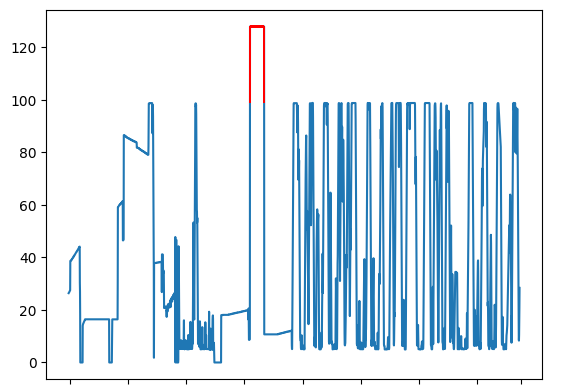
\includegraphics[width=0.5\linewidth]{figures/overflow-soc.png}
  \caption[Estado de carga excedente.]{Los valores del estado de carga excedente con respecto al limite operativo son registrados como inválidos por el protocolo.}
  \label{fig:overflow-soc}
\end{figure}

Con esto, se debe mencionar que el sistema desarrollado hace uso tanto de las señales a través de \textit{polling}, como de las señales espontáneas (asíncronas), aunque de forma más reducida en el caso de estas últimas. Concretamente, estas son configuradas para dar opción a la herramienta de optimización a conocer señales relacionadas con la disponibilidad de los recursos, y es que puede que el \gls{bess} haga saltar una alarma en caso de que se pierdan suficientes módulos de carga para afectar a la disponibilidad.

En el contexto del sistema desarrollado, el protocolo IEC 60870-5-104 es el canal de comunicación principal entre el \gls{rtu}, que actúa como servidor IEC 60870-5-104, y el \gls{pis}, que actúa como cliente. Esta comunicación es fundamental para transmitir los datos operativos de los activos energéticos al historiador de datos y, a su vez, para enviar las consignas de operación, los comandos de carga y descarga, desde el sistema de optimización hacia la planta.

Precisamente, la elección absolutamente fundamental del uso del protocolo IEC 60870-5-104 se realiza debido no solo a la capacidad de mensajería orientada a eventos, sino, principalmente, a las consideraciones de cumplimiento con los estándares impuestos por la institución dueña de la red eléctrica pública, el \gls{tso}, parte de sus funciones detalladas según su identificador conocido como \gls{asdu} en la tabla~\ref{tab:funciones-de-aplicacion-red}.

Ellos detallan el uso del protocolo para garantizar la respuesta con respecto al intercambio de información de la red. Por lo tanto, el sistema desarrollado se limita a seguir con la utilización de los estándares impuestos. De esta forma, se muestran para enfatizar el razonamiento industrial real por detrás de la decisión tomada del uso de IEC 60870-5-104, el cual está incluso ratificado oficialmente en España~\cite{une2017equipos}.

\begin{table}[ht]
  \centering
  \begin{tabular}{|l|p{7.5cm}|l|l|}
    \hline
    ASDU & Descripción                                               & Mnemónico   & Prioridad \\
    \hline
    103  & Sincronización del reloj                                  & C\_SC\_NA\_1 & Alta     \\
    147  & Programa de consumo                                       & M\_PC\_AA    & Baja     \\
    149  & Datos de tiempo real (Consumo)                            & M\_TR\_AA    & Baja     \\
    155  & Datos de tiempo real (Generación)                         & M\_TR\_GN    & Baja     \\
    169  & Orden de reducción de potencia                            & C\_PR\_IK    & Alta     \\
    180  & Petición de programa de consumo o de parada/mantenimiento & C\_PC\_AA    & Baja     \\
    182  & Petición de datos de tiempo real                          & C\_TR\_AA    & Baja     \\
    \hline
  \end{tabular}
  \caption[Funciones de aplicación para la comunicación con la red eléctrica.]{Extracto de las funciones de aplicación asociadas definidas por el operador del sistema de transporte para la comunicación del sistema con la red eléctrica, consolidadas en el llamado \gls{sceci}~\cite{ree2009protocolo}. El sistema hace uso de sus propias funciones de aplicación asociadas, comunicadas en última instancia a la red a través aquí mostrados.}
  \label{tab:funciones-de-aplicacion-red}
\end{table}

\section{Sistema de información de planta}
\label{makereference3.4}

Conociendo ya tanto los activos físicos disponibles, de los cuales obtener los datos sensoriales, como los canales de comunicación, es necesario ofrecer una interfaz de interacción bidireccional entre la herramienta principal que realiza la optimización operativa y la infraestructura física.

Para esta función crítica, la arquitectura del sistema se apoya en parte de la infraestructura preexistente del \gls{pis} desplegado.

Precisamente, en muchas arquitecturas de sistemas industriales reales en producción, la totalidad de la información entrante y saliente de los activos físicos pasa por el sistema SCADA\@. En cambio, aunque en la arquitectura general del desarrollo propio sí que tenga cabida uno de esos sistemas, la comunicación con los activos físicos es realizada sin ningún tipo de indirección secundaria, significando que el sistema SCADA queda fuera del alcance y no es pertinente al diseño realizado. Es decir, la información fluye directamente al \gls{pis} sin pasar por el SCADA\@, aunque exista un sistema SCADA externo.

\subsection{Contextualización del sistema}
\label{makereference3.4.1}

De esta forma, el \gls{pis} seleccionado se trata del llamado PI System de AVEVA (antes OSIsoft), una plataforma tecnológica diseñada para la gestión de datos de operaciones en tiempo real a escala industrial, que viene como anillo al dedo al caso de uso del sistema~\cite{aveva2025aveva}.

Su núcleo principal, el PI Server, actúa como un repositorio centralizado que no solo almacena, sino que también enriquece y contextualiza los extensos flujos de datos de series temporales provenientes de la instrumentación de campo.

Si bien el componente del servidor en concreto ya se encontraba desplegado, entendiblemente para controlar el resto de instalaciones no relacionadas con los \gls{bess}, su alcance no se extendía a la monitorización y control de los activos energéticos específicos pertinentes al desarrollo realizado, las instalaciones con activos de almacenamiento, concretamente.

Por lo tanto, una contribución fundamental resulta ser el diseño, la implantación y la configuración detallada de los canales de comunicación bidireccionales usando los componentes descritos anteriormente para integrar estos activos, detallado el diseño en la figura~\ref{fig:sistema-de-informacion-de-planta}.

\begin{figure}
  \centering
  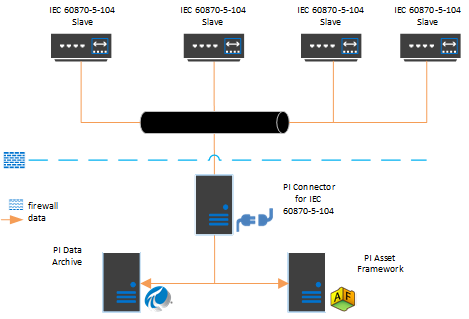
\includegraphics[width=0.5\linewidth]{figures/sistema-de-informacion-de-planta.png}
  \caption[Arquitectura del sistema de información de planta.]{Arquitectura de los canales de comunicación del sistema de información de planta~\cite{aveva2025aveva}.}
  \label{fig:sistema-de-informacion-de-planta}
\end{figure}

Para ello, se ha desplegado el PI Connector para IEC 60870-5-104, un componente de software que actúa como traductor entre el protocolo de telecontrol estándar del sector eléctrico y el ecosistema del PI System, también mostrado en la figura.

\subsection{Consideraciones de seguridad}
\label{makereference3.4.2}

Es bien sabido que las consideraciones de seguridad no son una característica más de los sistemas críticos industriales que controlan activos energéticos, sino que deben ser tomados como requerimientos fundamentales.

Por ello, el proceso de puesta en marcha requiere de una configuración precisa para garantizar, por una parte, la integridad de los datos y, por otra, su seguridad. Con esto, el conector es desplegado en un servidor Windows Server 2022 dedicado dentro de una llamada \gls{idmz}, asegurando la independencia y seguridad de las comunicaciones.

Las \gls{idmz} se encuentran entre las redes de \gls{ot} y de \gls{it} y se diferencian en que deben intentar asegurar la disponibilidad y los tiempos de respuesta de los procesos físicos industriales que alojan. Esto se traduce en que no se alojan necesariamente cerca de las fuentes de datos de campo, ni directamente junto al resto de servicios informacionales, sino que deben existir en las localizaciones relacionadas con la sala de control que supervisa el funcionamiento correcto de dichos servicios con por lo menos una seguridad mínimamente mayor.

Como tanto el conector como el servidor del \gls{pis} se encuentran en la misma \gls{idmz} y no en una red \gls{ot} en contrapunto a la red \gls{it}, no es necesario introducir otra capa de indirección. Esta capa actuaría como intermediario seguro para respetar las políticas de seguridad entre las redes, pero eso significa que debe existir un control en forma de \textit{firewall} más avanzado aún entre redes para que la herramienta de optimización pueda acceder al historiador (el \gls{pis}), en forma del llamado PI Relay. Aún así, gracias a la arquitectura usada, no es necesario introducir esta complejidad añadida a costa del aisaliento total entre redes (se sigue manteniendo el aislamiento necesario).

De esta forma, se observa que, en concreto, el despliegue del conector, actuando como \textit{gateway} entre el protocolo de comunicación y el historiador de datos, y precisamente el historiador de datos mismo, se encuentran posicionados en el nivel 3.5 de la zona desmilitarizada industrial de la \gls{pera}, el cual define un modelo estructural estandarizado para la seguridad de los sistemas de control industrial.

\begin{figure}
  \centering
  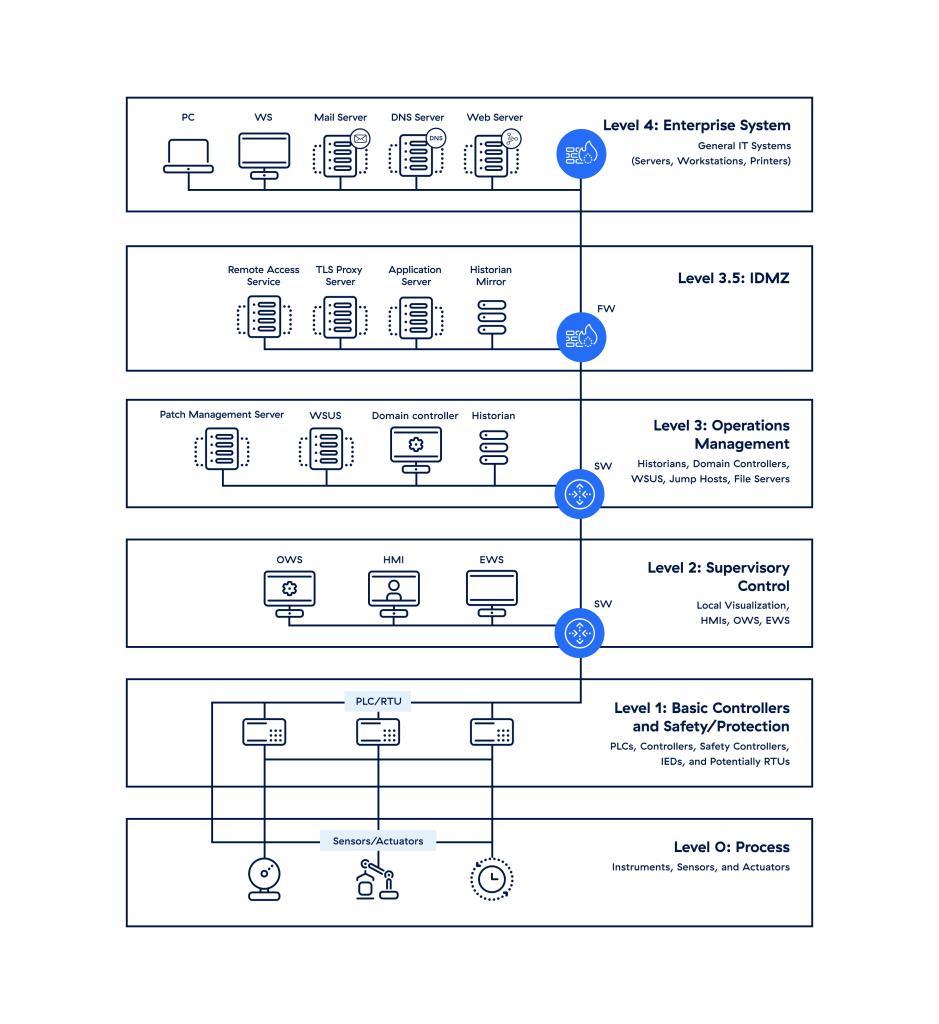
\includegraphics[width=0.5\linewidth]{figures/modelo-purdue.png}
  \caption[Modelo Purdue.]{Modelo Purdue para la seguridad de los sistemas de control industrial~\cite{zscaler2025what}.}
  \label{fig:modelo-purdue}
\end{figure}

\subsection{Configuración funcional}
\label{makereference3.4.3}

La parametrización del conector, junto con la especificación de parte la lógica de traducción a llevar a cabo, se ha realizado mediante el administrador del conector mostrado en la figura~\ref{fig:administador-del-conector}.

\begin{figure}
  \centering
  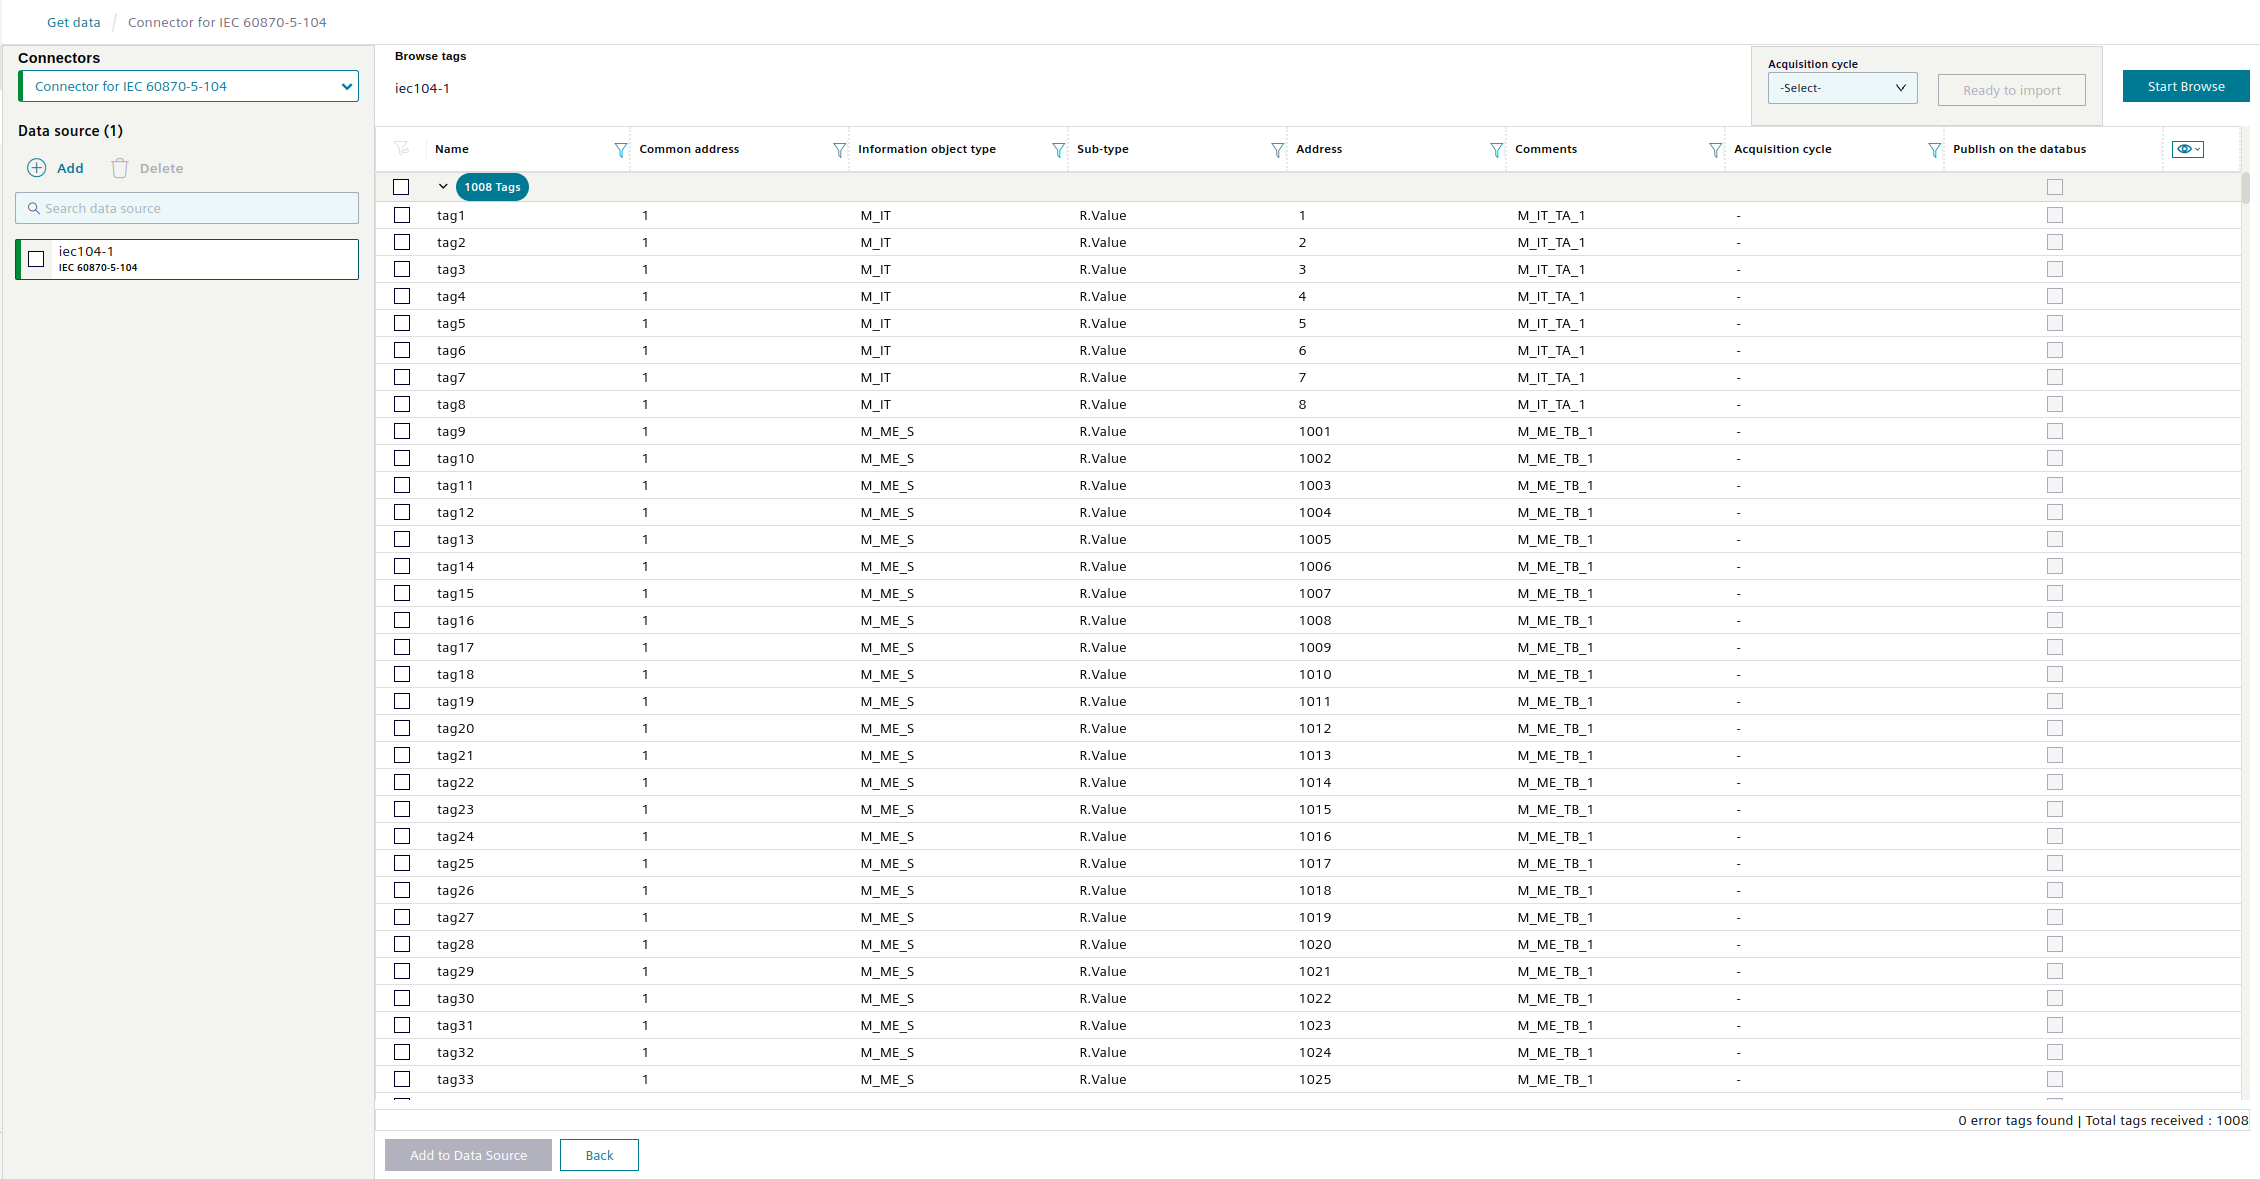
\includegraphics[width=0.75\linewidth]{figures/administador-del-conector.png}
  \caption[Interfaz del administrador del conector.]{Interfaz del administrador del conector mostrando el descubrimiento de señales del dispositivo subordinado.}
  \label{fig:administador-del-conector}
\end{figure}

Por la parte de la selección del PI Server al cual transmitir los datos, se especifica la dirección IP y el puerto del mismo. En concreto, el tipo de servidor se debe corresponder con la tecnología de archivado del historiador usada, la cual resulta ser PI Data Archive, a diferencia de PI Asset Framework de más alto nivel.

Desde la perspectiva de la fuente de datos, se requiere introducir la localización del dispositivo primario subordinado de IEC 60870-5-104.

Junto a ello, se ajustan los parámetros clave del protocolo en sí, como las \glspl{asdu}, que identifican unívocamente a la estación. Para facilitar el descubrimiento, es posible enviar un comando de \gls{gi} utilizando la \gls{asdu} 0xFFFF que devuelva todos los canales encontrados en el dispositivo subordinado, y filtrarlos posteriormente.

A su vez, para garantizar un tiempo de respuesta razonable, se configuran también los temporizadores del protocolo. El temporizador \( t_1 \) determina el timeout de la confirmación de datos enviados, el \( t_2 \) el timeout de envío del reconocimiento si no se han enviado datos nuevos, y el \( t_3 \) el timeout de inactividad de la conexión.

Como el servicio de ajuste obligatorio (no remunerado) con menor granularidad es de 30 segundos máximo, es decir, se deben enviar pulsos que cubran el 50 \% de la regulación en menos de 15 segundos y el 100 \% en menos de 30 segundos para controlar la batería~\cite{cnmc2024balance}, es necesario aplicar valores menores o iguales a dichos tiempos a los temporizadores \( t_1 \) y \( t_2 \), 4 segundos según recomendaciones, concretamente.

Es importante recalcar que aunque la menor granularidad a la que deben trabajar las baterías sea tan baja, el sistema desarrollado nunca necesitará de un tiempo de respuesta tan rápido, ya que controla el arbitraje de batería en mercados de más alta granularidad (mayor o igual a 15 minutos). Tan solo se modifican los temporizadores para, de forma ajena al desarrollo, tener la opción de habilitar los sistemas de almacenamiento de energía en batería no solo para el uso del sistema propio, sino para el negocio simultaneo en los mercados auxiliares previamente descritos y servicios de regulación, que son los que disponen de esta granularidad reducida.

Finalmente, intentando asegurar la sincronización de los sensores y evitar la perdida de información, la periodicidad de la \gls{gi}, comando esencial del protocolo que solicita una actualización completa de todos los puntos de datos, se define en 1 hora. Esto es debido a que este valor se corresponde con el intervalo mínimo entre la negociación de dos mercados, lo que es diferente de la granularidad del mercado. Aún así, los búferes de transmisión de las unidades remotas permiten disminuir notablemente la perdida de datos. Esto es relevante ya que el sistema de control de planta no realiza peticiones bajo demanda a los dispositivos, sino que devuelve el valor ya al almacenado.

\begin{figure}
  \centering
  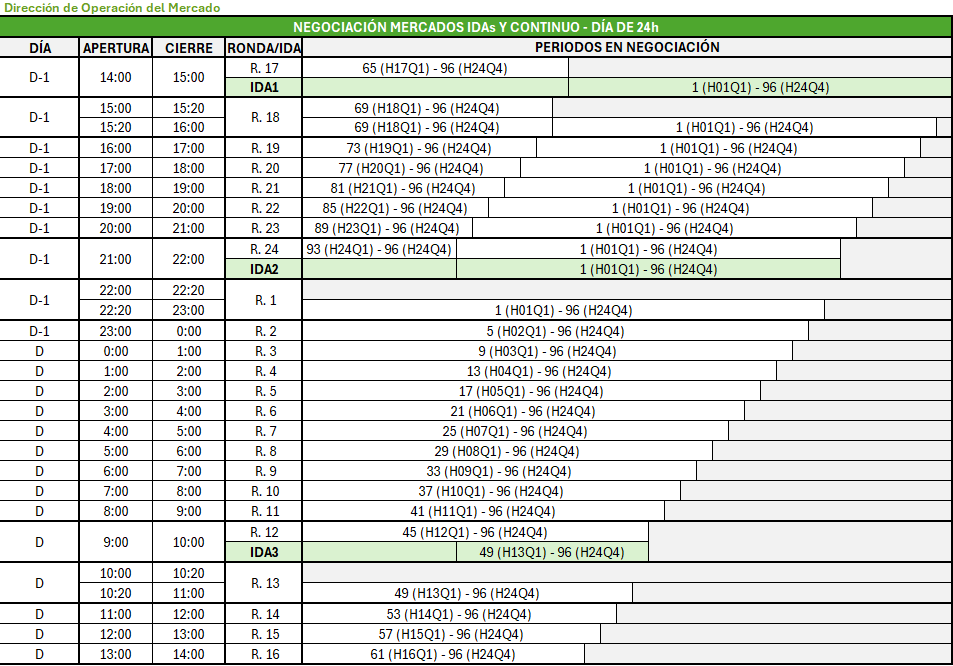
\includegraphics[width=0.75\linewidth]{figures/tiempo-mercados.png}
  \caption[Calendario de negociación de los mercados eléctricos.]{Calendario de negociación de los mercados eléctricos intradiarios y continuo~\cite{omie2025mercado}.}
  \label{fig:tiempo-mercados}
\end{figure}

Más allá y tal y como se ha descrito anteriormente, es posible aprovechar las capacidades de mensajería orientadas a eventos del protocolo para no tener que enviar comandos de \gls{gi} continuamente. No importa no tener datos estrictamente actualizados para las señales relacionadas con los parámetros operativos del \gls{bess}, pero sí que importa no estar actualizados en cuanto a su disponibilidad estructural. Es decir, parámetros como el \gls{soc}, la energía almacenada, la potencia de carga o descarga, etc.\ son modelados intrínsecamente en el funcionamiento de la instalación, en cambio, los fallos estructurales no lo son (pueden ocurrir en cualquier momento, el resto tienen comportamientos predecibles). Por suerte, una vez configurada la relación con los puntos de la conexión, el conector es capaz de recibir estas señales espontaneas automáticamente aprovechando el funcionamiento del protocolo.

De esta forma y una vez establecido el enlace de comunicación, el conector procede al descubrimiento de las señales disponibles, interrogando al controlador de planta y presentando una lista completa de los objetos de información accesibles, cada uno identificado por su dirección de objeto de información.

Se seleccionan únicamente las variables críticas para la operación de la batería y la planta de generación asociada, correspondientes a las señales de los sensores anteriormente descritos en la sección~\ref{makereference3.2}. Posteriormente, se debe realizar un mapeo explícito de cada \gls{ioa} seleccionada a un elemento de datos en el PI Server. Para cada señal, se crea un PI Point correspondiente en el PI Data Archive, definiendo sus atributos como tipo de dato (\texttt{Float32} para mediciones continuas, \texttt{Digital} para descripciones de estado), unidades de ingeniería (\si{\percent}, \si{\mega\watt}, \si{\mega\watt\hour}), un descriptor textual claro y el identificador correspondiente (\texttt{BT SOC Real}, etc.). Es posible visualizar el resultado en la figura~\ref{fig:visualizacion-industrial-de-batería}.

\begin{figure}
  \centering
  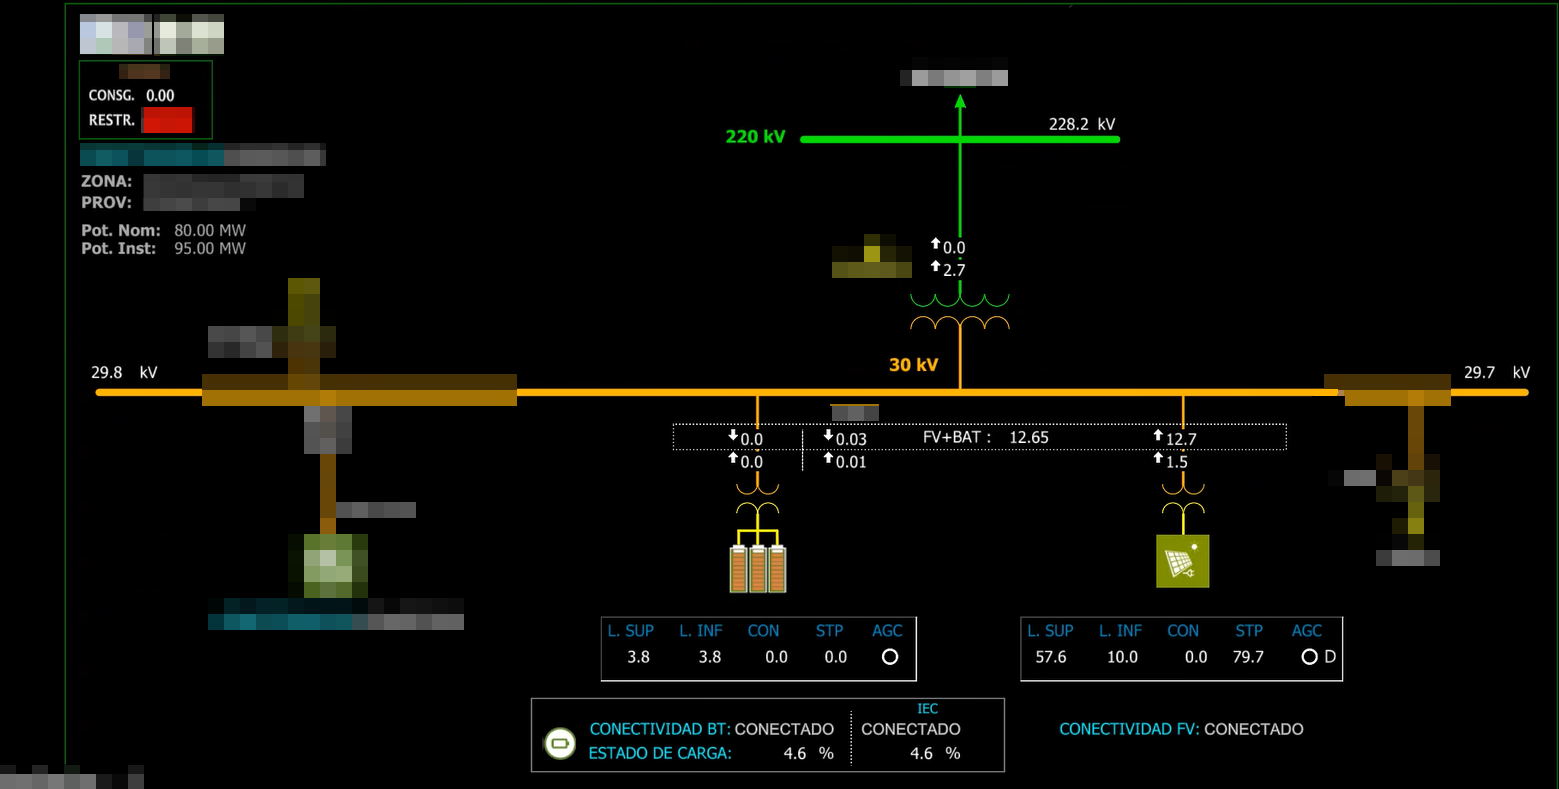
\includegraphics[width=0.75\linewidth]{figures/visualizacion-industrial-de-bateria.png}
  \caption[Visualización industrial de señales de instalación.]{Visualización industrial de varias señales de una instalación.}
  \label{fig:visualizacion-industrial-de-bateria}
\end{figure}

Como no se hace uso de PI Asset Framework para modelizar la planta de forma jerárquica, se definen los identificadores de cada punto según sus características. Los valores analógicos (analog value) siguen el formato \texttt{M:06X.AV}, las calidades analógicas (analog quality) \texttt{M:06X.AQ}, los valores de las consignas (setpoint value) \texttt{M:06X.SV} y las calidades de las consignas (setpoint quality) \texttt{M:06X.SQ}. Se muestra una colección de los mismos en la tabla~\ref{fig:puntos-bateria}.

\begin{figure}
  \centering
  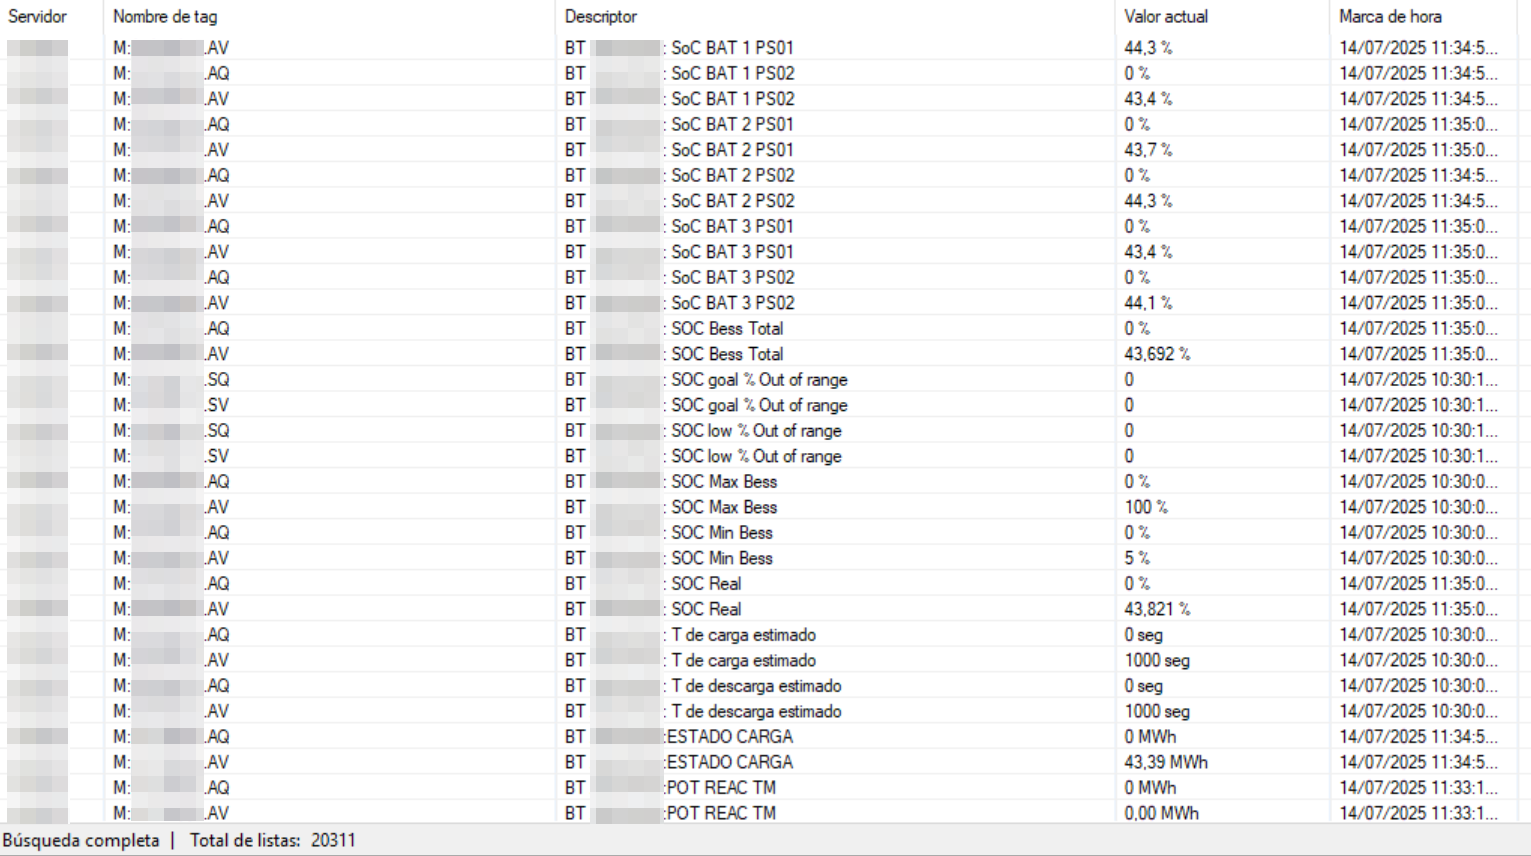
\includegraphics[width=0.75\linewidth]{figures/puntos-bateria.png}
  \caption[Colección de puntos de una batería.]{Colección de puntos de una batería.}
  \label{fig:puntos-bateria}
\end{figure}

Los valores, como su nombre indica, se corresponden con el contenido de las señales, sean continuas o no. Las calidades, en cambio, representan la salud de las señales definido por el protocolo y son usadas para filtrar malas señales.

Con ello, la validación del sistema se realiza comparando en tiempo real los valores registrados en el PI Data Archive con las lecturas directas en la interfaz SCADA de los controlador de planta en la respectiva sala de control securizada, y forzando cambios en los activos para verificar la correcta transmisión y registro de eventos. De esta forma, es posible comparar el programa de carga y descarga de las baterías con los movimientos verdaderamente efectuados y comprobar su corrección, como se muestra en la figura~\ref{fig:programa-bateria}.

\begin{figure}
  \centering
  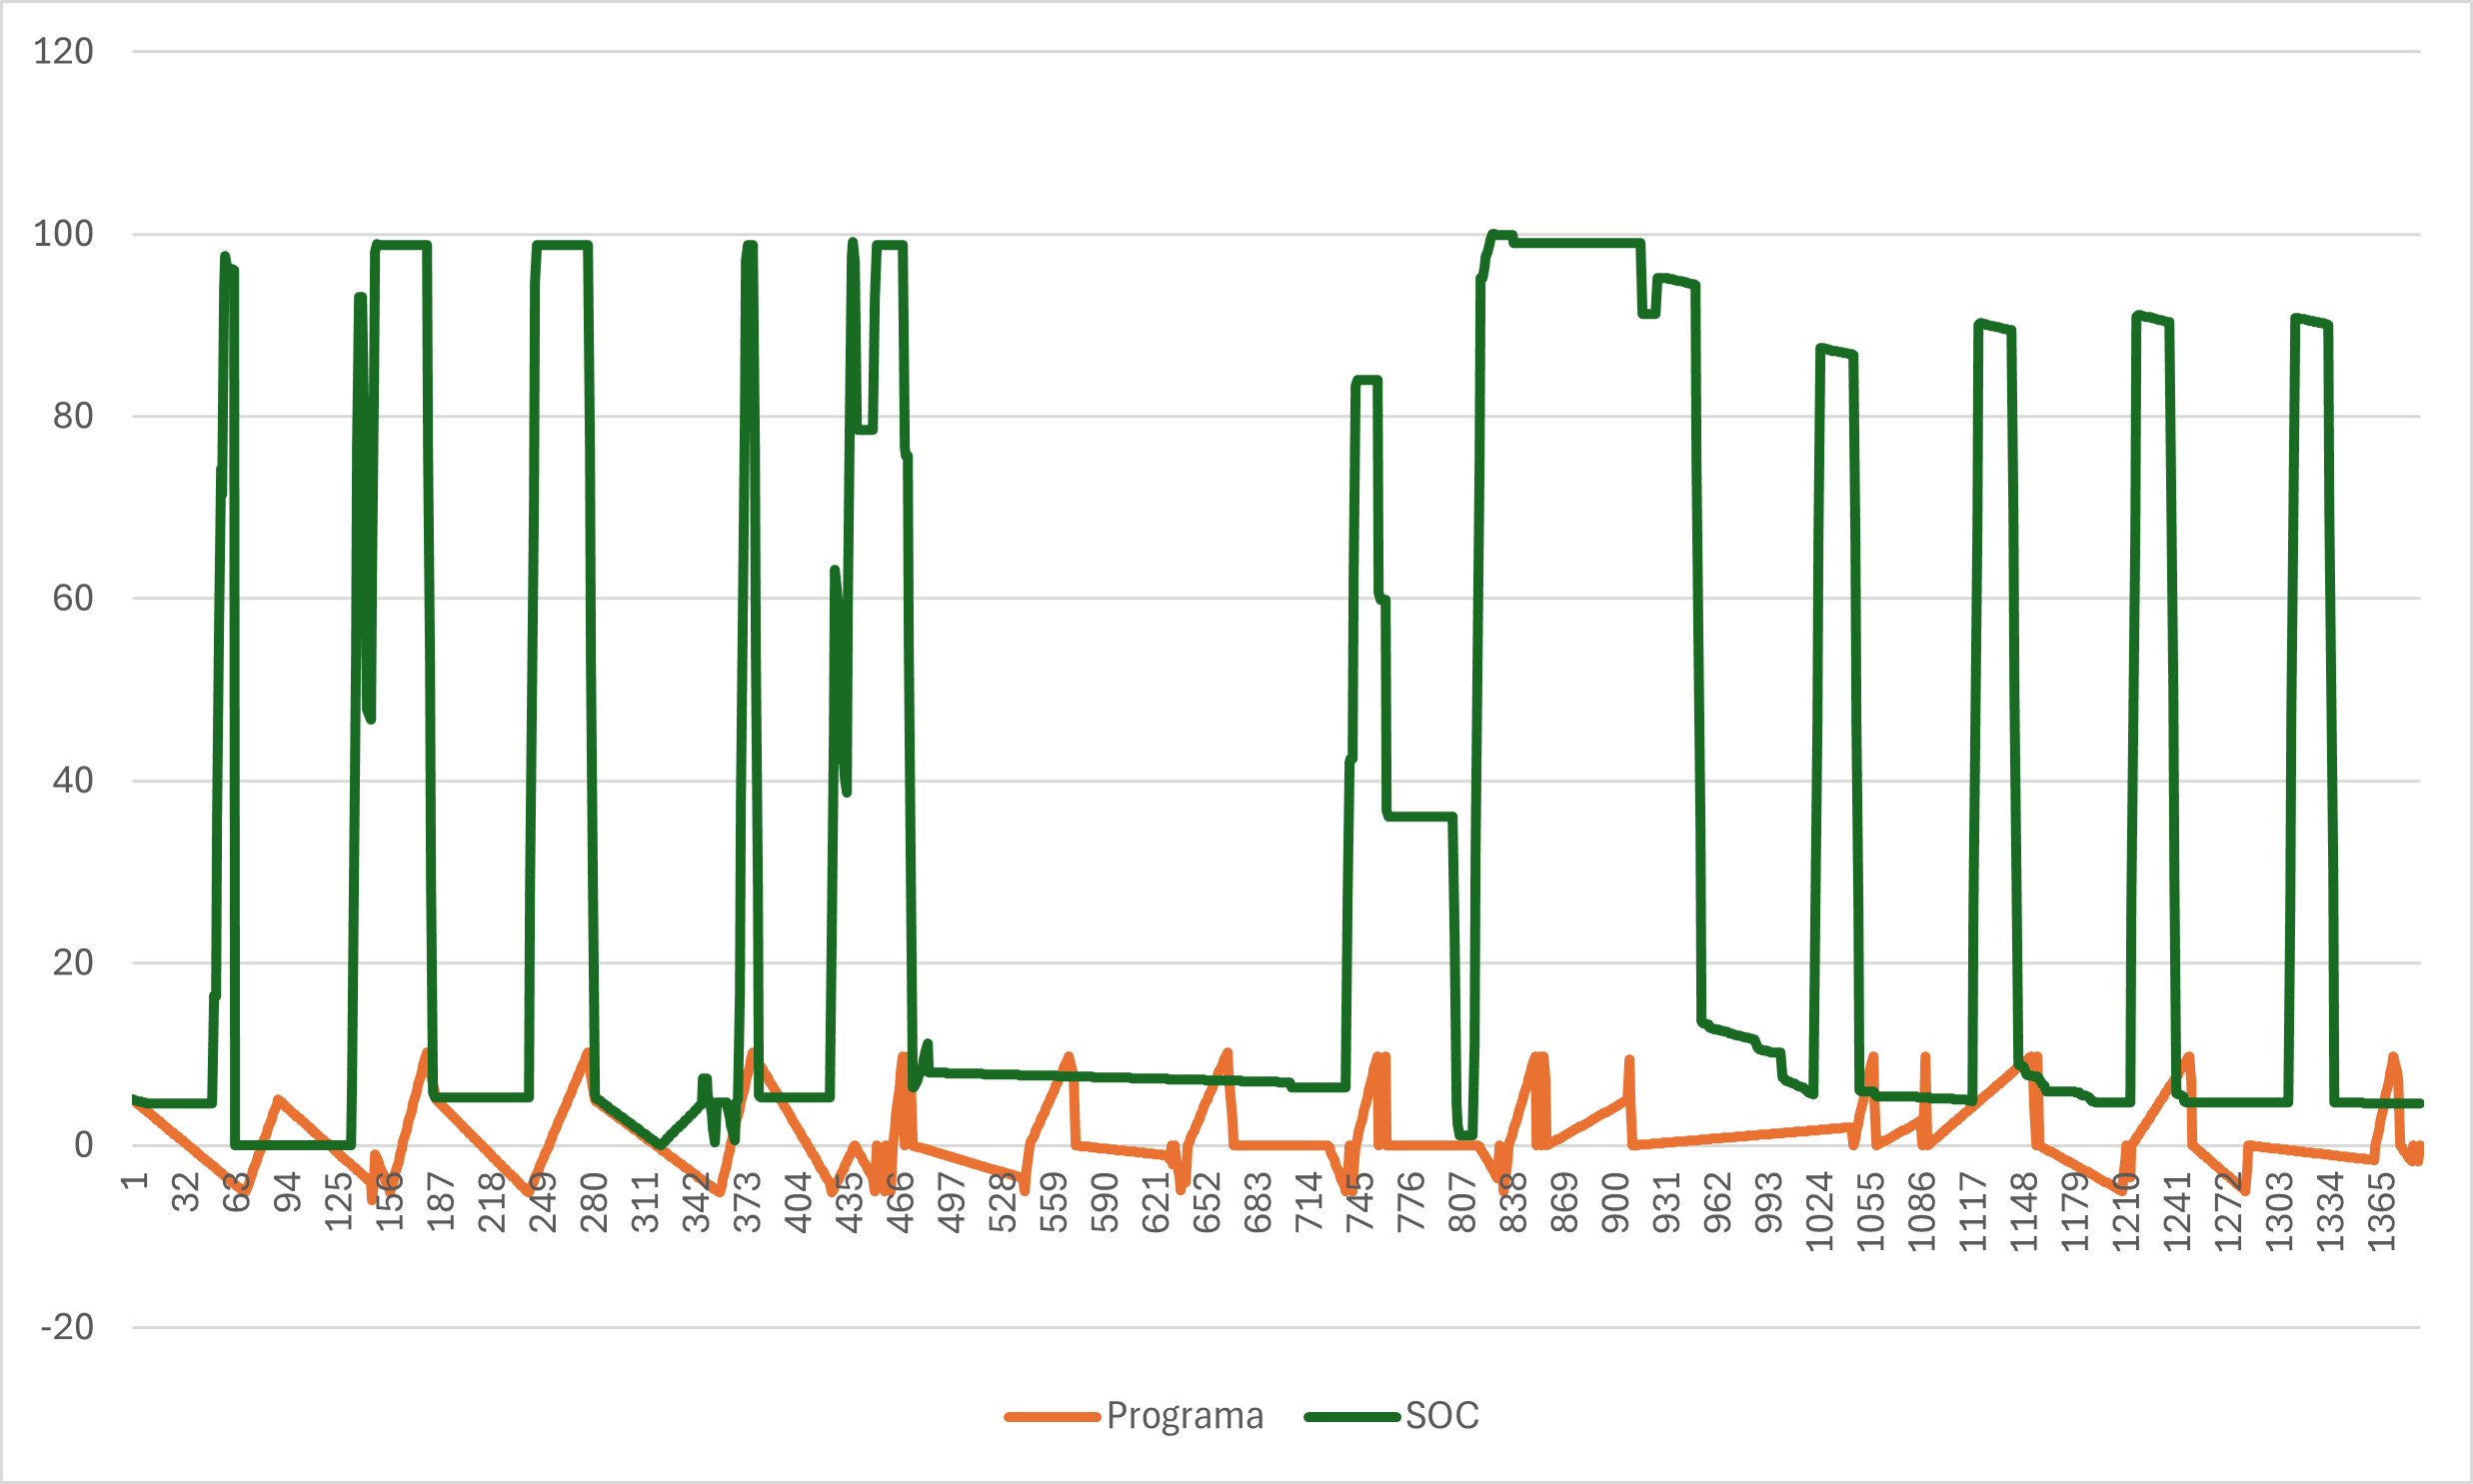
\includegraphics[width=0.75\linewidth]{figures/programa-bateria.png}
  \caption[Programa de ciclado de una batería.]{Programa de ciclado de una batería en comparación con su evolución del estado de carga.}
  \label{fig:programa-bateria}
\end{figure}

Precisamente, esta validación permite determinar múltiples errores en la lógica de consignación, De hecho, durante la validación se consiguieron corregir múltiples fallos más o menos críticos.

Uno de ellos, el hecho de olvidarse bajar la potencia de las baterías al mínimo técnico tras el mandato de una señal de carga, error que precisamente causa una carga excedente de la baterías durante el periodo de pruebas correspondiente a una perdida monetaria puntual del calibre de miles de euros netos.

Otra situación interesante fue dada por el método de actualización de las señales de \textit{polling} y las espontaneas, como la disponibilidad. Como la disponibilidad es actualizada nada más cambiar, por consideraciones de reporte, puede que no se encuentren sincronizadas con las otras señales. Para resolverlo, se ponen en acuerdo la disponibilidad y el resto de señales relacionadas con la misma una vez se haya realizado la petición.

Por suerte, el sistema de control de baterías no permite el incorrecto funcionamiento de las baterías desde la perspectiva física y hace sonar la alarma ante tales situaciones, actualizando su disponibilidad, por lo que la batería no sufre ningún daño aunque no se disponga de recurso energético en periodos de carga.

\section{Consumo del historiador}
\label{makereference3.5}

Una vez que la infraestructura de adquisición y almacenamiento ha sido configurada y validada, y los datos operativos de los activos fluyen de manera fiable hacia el historiador, el siguiente paso es establecer los mecanismos para su consumo.

Precisamente, el consumo no se limita a una simple lectura de valores brutos, sino que abarca la transformación de algunas de las métricas para la obtención de valores dependientes, como los rendimientos del ciclo, y la interfaz programática que conecte el historiador con la herramienta de optimización, intentando hacer frente a posibles incompatibilidades tecnológicas entre ambas plataformas.

\subsection{Ecuaciones de rendimiento}
\label{makereference3.5.1}

Para representar valores dependientes con significado físico, en vez de tener que consultar múltiples puntos simultáneamente para inferir el resultado computado de los mismos, resulta más conveniente y efectivo el uso de las ecuaciones de rendimiento proporcionadas como parte del PI System.

Las ecuaciones de rendimiento o PI Performance Equations son una solución eficaz para detallar la lógica de señales calculadas de forma similar a la definición previa de los puntos. Precisamente, la diferencia principal es la introducción de la ecuación misma y el evento de actualización, ya que se requiere conocer de que puntos depende la ecuación para poder recomputarla cuando estos cambien.

\begin{figure}
  \centering
  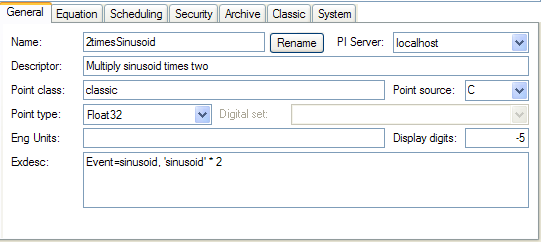
\includegraphics[width=0.5\linewidth]{figures/ecuaciones-de-rendimiento.png}
  \caption[Creación de una ecuación de rendimiento.]{Creación de una ecuación de rendimiento.}
  \label{fig:ecuaciones-de-rendimiento}
\end{figure}

Mediante las ecuaciones de rendimiento se detallan los siguientes puntos.

\begin{itemize}

  \item El rendimiento de carga, que afecta a la energía importada y define la cantidad de energía perdida durante la carga de la batería. Su razón de ser es el ajuste de los posibles desvíos a la hora de comprar energía que surgirían si no se tuvieran en cuenta las perdidas. El rendimiento de carga es calculado mediante la simple relación entre la energía importada y energía cargada \( \eta_{c} = E_{\text{imp}} / E_{c} \).

  \item El rendimiento de descarga, que afecta a la energía exportada y define la cantidad de energía perdida durante la descarga de la batería. Es necesaria para el ajuste de los posibles desvíos a la hora de vender energía si no se tuvieran en cuenta las perdidas. El rendimiento de descarga es calculado mediante la simple relación entre la energía exportada y energía descargada \( \eta_{d} = E_{\text{exp}} / E_{d} \).

\end{itemize}

\subsection{Integración programática}
\label{makereference3.5.2}

Finalmente, teniendo los datos provenientes de tanto de los activos físicos disponibles en el historiador como de sus propias transformaciones, es necesario consumirlos por la herramienta principal de optimización con el propósito de conocer los parámetros operativos de las baterías.

Para ello, existen múltiples enfoques que tomar, aunque el elegido a sido hacer uso de la interfaz de aplicación ofrecida por el PI AF SDK, la cual provee acceso estructurado a una variedad de componentes del PI System.

% TODO
\begin{figure}
  \centering
  % \includegraphics[width=0.5\linewidth]{figures/integración-programatica.png}
  \caption[Diagrama de componentes entre plataformas.]{Diagrama de componentes entre plataformas.}
  \label{fig:integración-programatica}
\end{figure}

Aún y todo, la librería expone su interfaz a través de Microsoft \.NET pero la herramienta de optimización ha sido desarrollada en Python, lo que resulta en un problema de incompatibilidad que podría no permitir el uso de PI AF SDK\@.

Para solucionar el problema principal de esta incompatibilidad, es posible utilizar la integración de Python con el \.NET Common Language Runtime, la máquina virtual que se encarga de ejecutar el código para la plataforma de \.NET\@. Esto se hace posible a través de los bindings de Python.NET\@.

Precisamente, se hace un uso directo de la interfaz a través del lenguaje de programación elegido para el apartado de la conexión con el PI Server. Y es que, en términos de la conexión, resulta que para cumplir con los requisitos de seguridad de la comunicación entre redes, los métodos de conexión por defecto recomendados no se pueden usar. En cambio, es necesaria la autenticación con credenciales directa, aunque esto suponga la perdida de la reconexión automática ofrecida por los métodos de conexión por defecto.

Junto a ello, con el propósito de aumentar la ergonomía del desarrollo, se toma la librería Piconnect, que ofrece una interfaz directa más simple y también hace uso internamente de la integración con la interfaz de \.NET, resultando en el diagrama de la figura~\ref{fig:integración-programatica}.

Con todo, los puntos son consumidos mediante los llamados valores registrados, significando un valor discreto en el tiempo, y valores interpolados, para obtener la evolución de los mismos a lo largo del tiempo. La comunicación de vuelta a los activos físicos es discutida más adelante en la sección correspondiente de comando y control~\ref{makereference6.1.1}.
